\documentclass[9pt,twocolumn,twoside]{../../styles/osajnl}
\usepackage{fancyvrb}
\journal{i524} 

\title{RabbitMQ}

\author[1,*]{Abhishek Gupta}

\affil[1]{School of Informatics and Computing, Bloomington, IN 47408, U.S.A.}

\affil[*]{Corresponding authors: abhigupt@iu.edu}

\dates{project-001, \today}

\ociscodes{Cloud, I524}

% replace this with your url in Github/gitlab
\doi{\url{https://github.com/cloudmesh/sp17-i524/blob/master/paper1/S17-IO-3005/report.pdf}}

\begin{abstract}
RabbitMQ provides messaging platform which allows applications pass messages in
a reliable and fault tolerant way. RabbitMQ implements Advanced Message Queuing
Protocol (AMQP) and is written in Erlang programming language. It runs on all
major operating systems and supports SDK in all major programming
languages\cite{www-rabbitmq-develop} including objective-C, swift and node.js.
When we look for messaging, we look for certain features: asynchronous
messaging, large scale, reliability, clustering, multi-protocol, highly
available, fault tolerant. RabbitMQ\cite{www-rabbitmq-pivotal} fulfills these
requirements and provides a distributed, persistent, highly available, fault
tolerant messaging system which can scale as data grows.
\end{abstract}

\setboolean{displaycopyright}{true}

\begin{document}

\maketitle

\section{Introduction}
RabbitMQ \cite{www-rabbitmq-pivotal} based off AMQP (Advanced Message Queuing
Protocol\cite{vinoski2006advanced}) Which defines how client applications
connect to message brokers. Message brokers receive messages from producers and
make it available to consumers. The producer posts messages to exchanges and
broker agent read these messages from the exchange and write to queues.
Consumers can further read messages from the queue. It also supports a notion of
acknowledgments where consumers can post an acknowledgment back to broker and
which in turn can post messages back to the producer. Broker plays an important
role, it eliminates the well-known producer-consumer problem
\cite{www-producer-consumer-wiki}. It also provides persistence in case of
failures.

Looking back at the history \cite{videla2012rabbitmq} of the development of
RabbitMQ, it started with IBM Miseries in 1993, 1997 Microsoft MQ, 2001 java
messaging service. These technologies were incubated in different companies with
a common goal to create a messaging service for a distributed system. It was
then in 2003 where JP Morgan created the first version AMQP which became the
base for RabbitMQ technologies formed in 2006.

\begin{figure}[htbp]
\centering
\fbox{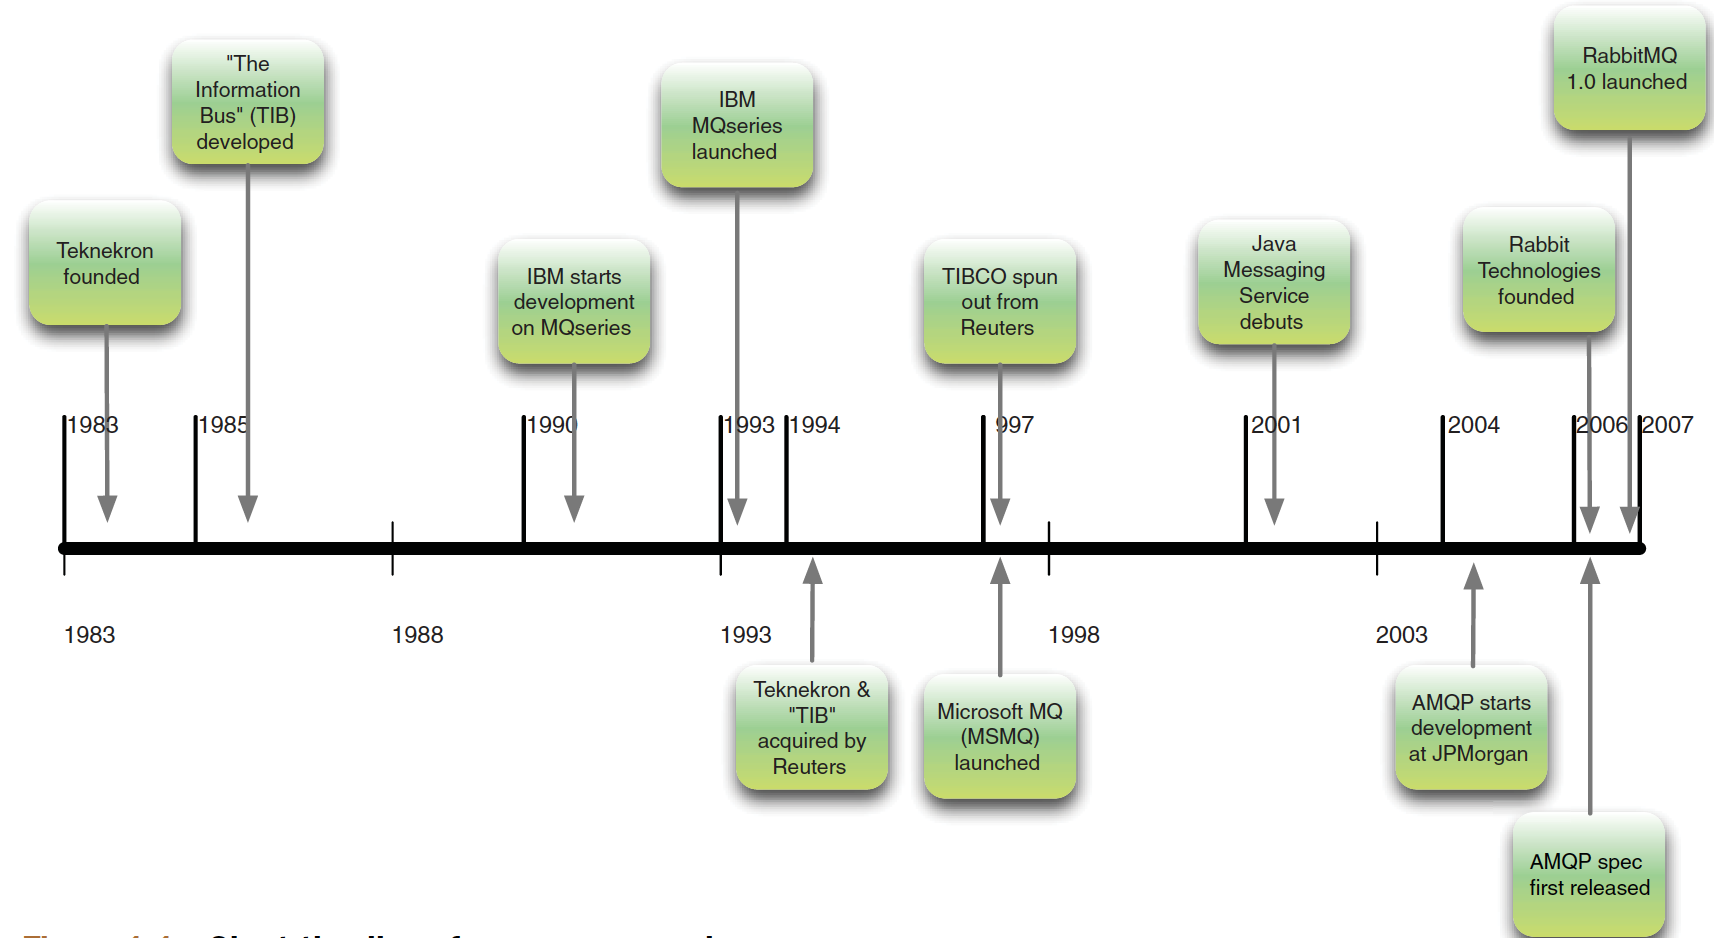
\includegraphics[scale=0.2]{images/mq_timeline}}
\caption{Timeline for evolution of RabbitMQ \cite{videla2012rabbitmq}}
\label{fig:false-color}
\end{figure}

\section{Architecture}
At high level, producers publish messages to the broker. Consumers consume
messages from the broker. Broker acts like a middle man, who has knowledge of
all available exchanges and queues \cite{videla2012rabbitmq}. It maintains
bindings between exchanges and queues. Exchanges here are often compared to post
offices or mailboxes.  Following table shows different type of exchanges
supported by RabbitMQ and corresponding default exchanges
\cite{www-rabbitmq-pivotal} .

An exchange is a binding to queue(s). So when you send a
message to an exchange, the broker checks the routing key of the message
and compares it against the queue bindings. Further it sends the message to
appropriate queue.

\begin{center}
 \begin{tabular}{||c c||} 
 \hline
 Name & Default pre-declared names \\ [0.5ex] 
 \hline\hline
 Direct exchange & (Empty string) and amq.direct  \\ 
 \hline
 Fanout exchange & amq.fanout  \\
 \hline
 Topic exchange & amq.topic  \\
 \hline
 Headers exchange & amq.match (and amq.headers in RabbitMQ) \\
 \hline
\end{tabular}
\end{center}

\section{Type of exchanges}
\label{sec:examples}

The sections below explains various types of exchanges supported by RabbitMQ.

\subsection{Default Exchange}
It is created by the broker and all queues are bound to default exchange unless 
specified separately. For example we have a queue called demoqueue, all messages 
assigned to demoqueue will be routed by default exchange.

\subsection{Direct exchange}
It is used to route messages to queue with a given routing key. For example a 
message queue has routing key K. A message with same routing key K will be 
delivered to same message queue.

\subsection{Fanout exchange}
Delivers messages to all queues bound to a given exchange. Fanout exchange
ignores the routing key. For example, if there are 5 queues bound to an exchange
'E'.  Messages to exchange 'E' are delivered to all 5 queues.

\subsection{Topic exchange}
It delivers messages to a given queue, not just based on the routing key but a
pattern specified in the message. This pattern is called topic. It can be useful
in scenarios where consumer decides which topic(s) it is interested in.
Further, it can subscribe to those topic(s).

\subsection{Header exchange}
This exchange ignores the routing key but rather uses a header parameter to
decide which message goes to which queue. A message is matched when a value in
header matches with the one specified in the queue binding. Exchanges have other
important attributes apart from routing key and exchange type. For example,
name, durability, auto-delete, arguments etc. Durability allows messages to
persist on disk in case broker restarts. Auto-delete deletes the exchange once
all queues have finished using the exchange.

\begin{figure}[htbp]
\centering
\fbox{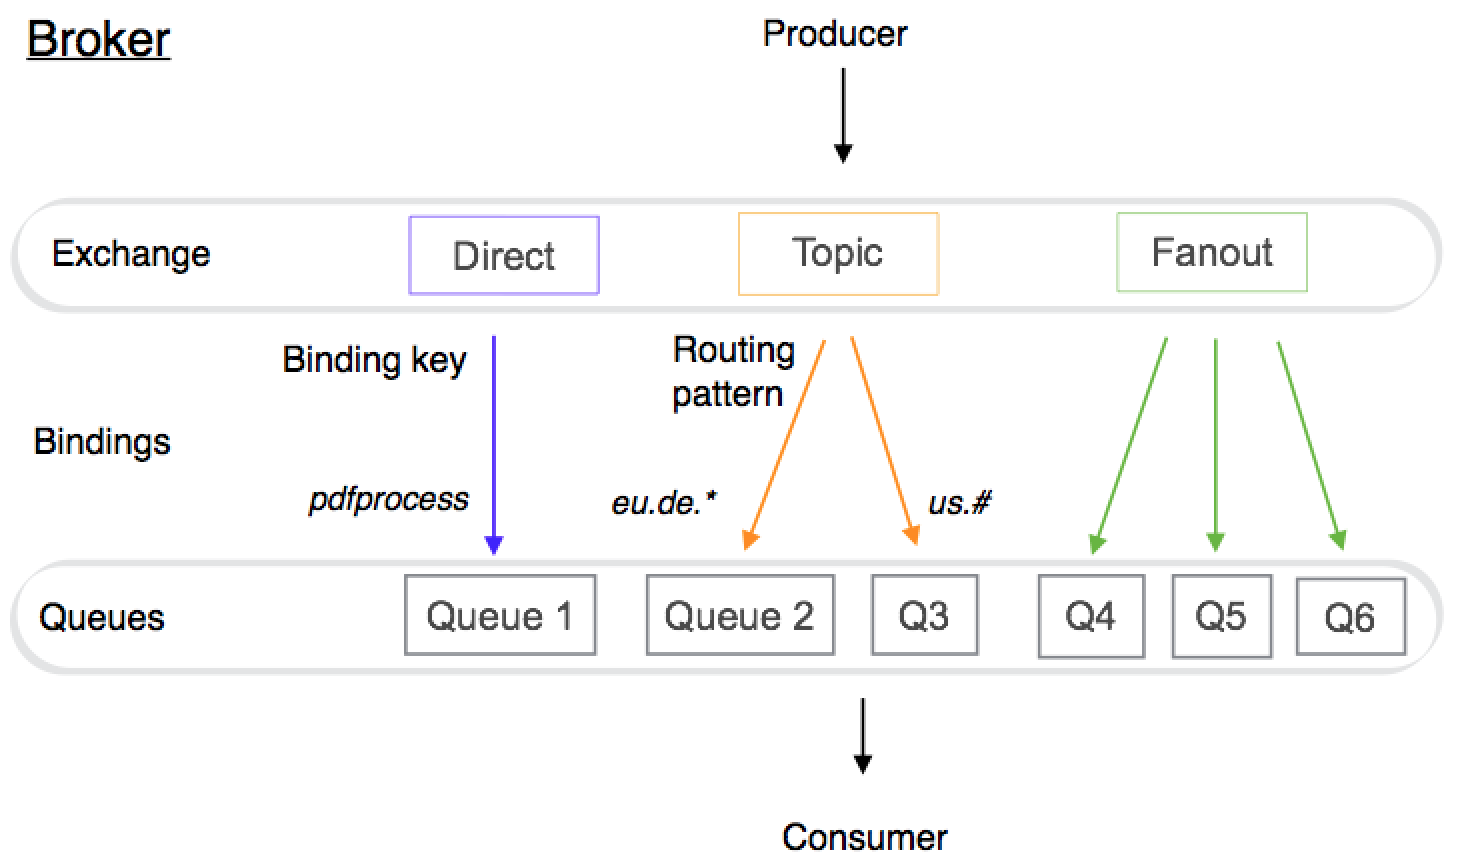
\includegraphics[scale=0.3]{images/exchanges-topic-fanout-direct}}
\caption{Different type of exchanges supported by
RabbitMQ\cite{www-rabbitmq-Johan}}
\label{fig:false-color}
\end{figure}

\section{Bindings}
Binding is a rule that defines how exchanges will route messages to the queue.
To route all messages from an exchange E to queue Q, Q has to be bound to
Exchange E. Binding uses routing key as one of the criteria to route messages to
a queue. However, routing key is optional and not always applicable.

\section{Consumers}
Messages from message queue are eventually used or consumed by consumers.
Consumers can use push or pull mechanism to consume these messages. Push API
have messages delivered to the consumer whereas a Pull API is used to fetch
messages from the queue. 

\section{Message Acknowledgement}
RabbitMQ has a built-in mechanism to send and receive acknowledgements. Producer
can send a message and wait for the acknowledgement in the response queue of the
consumer.  Once consumer successfully receives the message, it can post an
acknowledgement to the response queue. Here request queue and request exchange
can be used to send and receive messages. Response queue and response
exchange can be used to send and receive acknowledgements. This mechanism makes
RabbitMQ robust to handle failure scenarios.

\section{Clustering}
To achieve high availability \cite{videla2012rabbitmq} and making sure producers
and consumers send and receive data without knowing about node failures,
clustering was introduced. RabbitMQ follows OTP(open telecom platform) framework
provided by erlang to achieve high availability. RabbitMQ by default doesn't
replicate the content of queues i.e. all queues are stored on one node in the
cluster. To achieve clustering RabbitMQ keeps track of metadata for queue,
exchange, binding and vhost. In case of cluster mode, where broker, producer and
consumer run on different nodes, RabbitMQ only stores information about the
queue like metadata, state and contents on one node rather than all nodes on the
cluster. However, it stores metadata and pointer to actual data on each node on
the cluster. This is to optimize storage space and performance. 

\begin{figure}[htbp]
\centering
\fbox{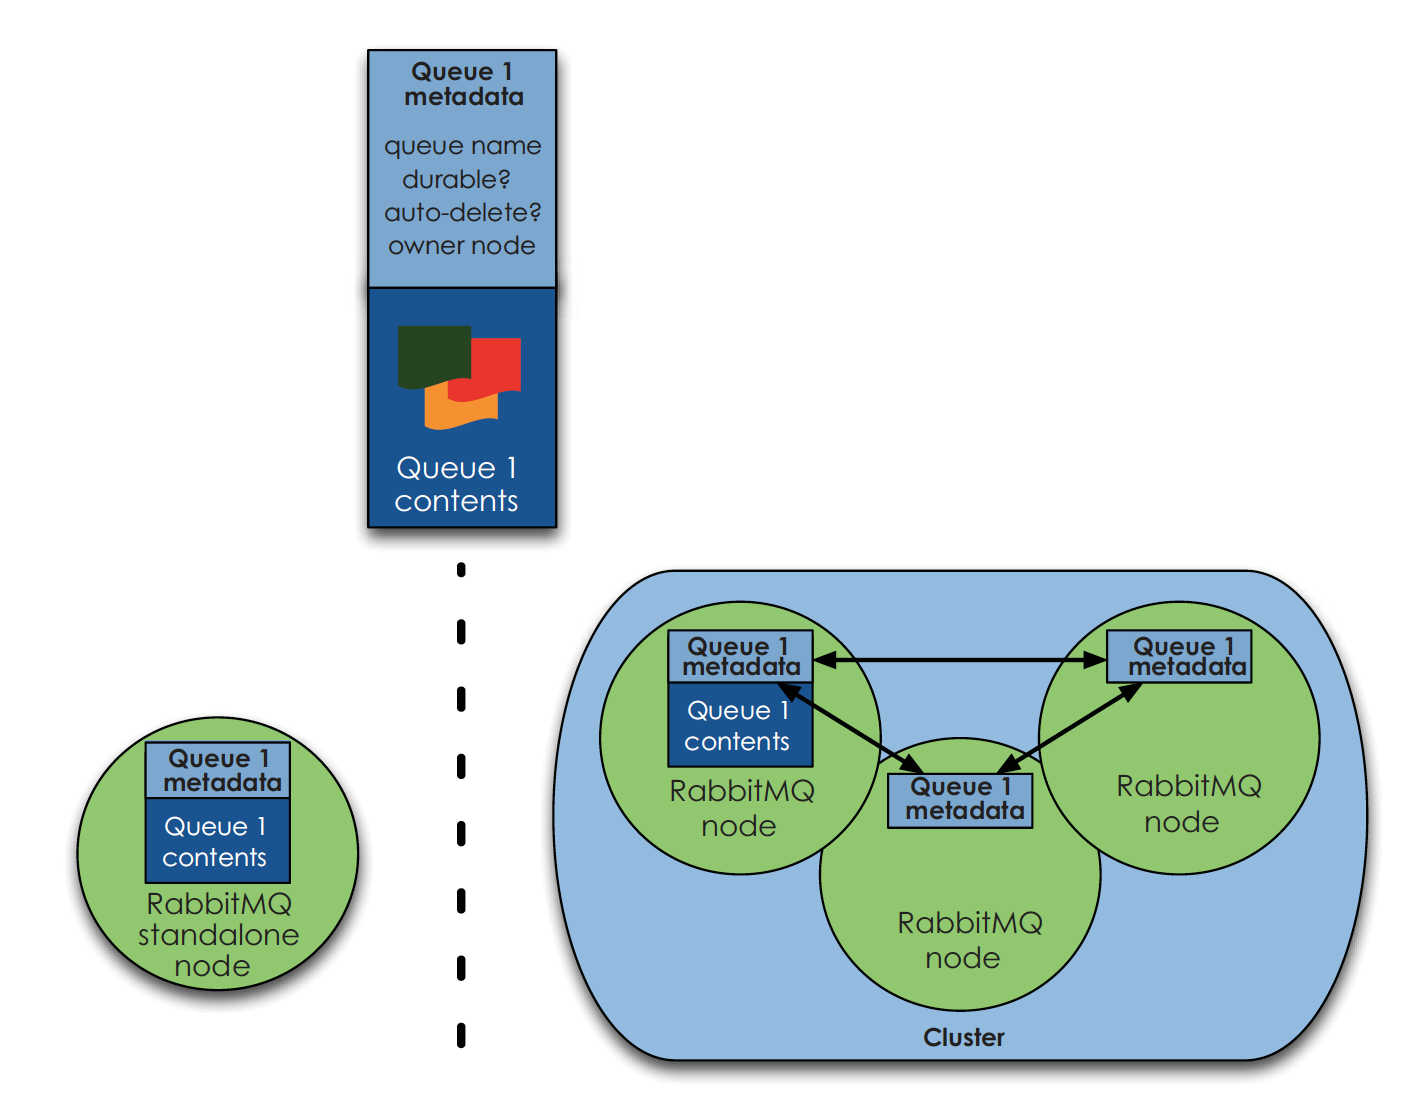
\includegraphics[width=\linewidth]{images/clustering-queue-metadata}}
\caption{Shows queue metadata for a cluster vs single node \cite{videla2012rabbitmq}}
\label{fig:false-color}
\end{figure}

Since, exchanges act like lookup tables for queue bindings, they are replicated
across all nodes on the cluster. 

\section{Management}
RabbitMQ provides all management using:
\begin{itemize}
	\item Web UI 
	\item REST interface
	\item rabbitmqctl command line utility
\end{itemize}

Web UI can be used by the administrator to create user, monitor queues and
exchanges, view statistics, add configurations etc. Similar functionality can be
achieved by CLI(command line interface) utility called rabbitmqctl or using REST
API. Rabbitmqctl can be used to automate RabbitMQ deployments and management. It
can also be used to write automated tests. REST API can be used for integrating
with 3rd part UI and plugins.  Using REST API, you can monitor the number of
connections, download or upload a configuration, list the nodes in the cluster,
create or delete RabbitMQ users, view or create virtual host, set permission for
a user etc. You can also list all current APIs using '/api' URI.

\begin{figure}[htbp]
\centering
\fbox{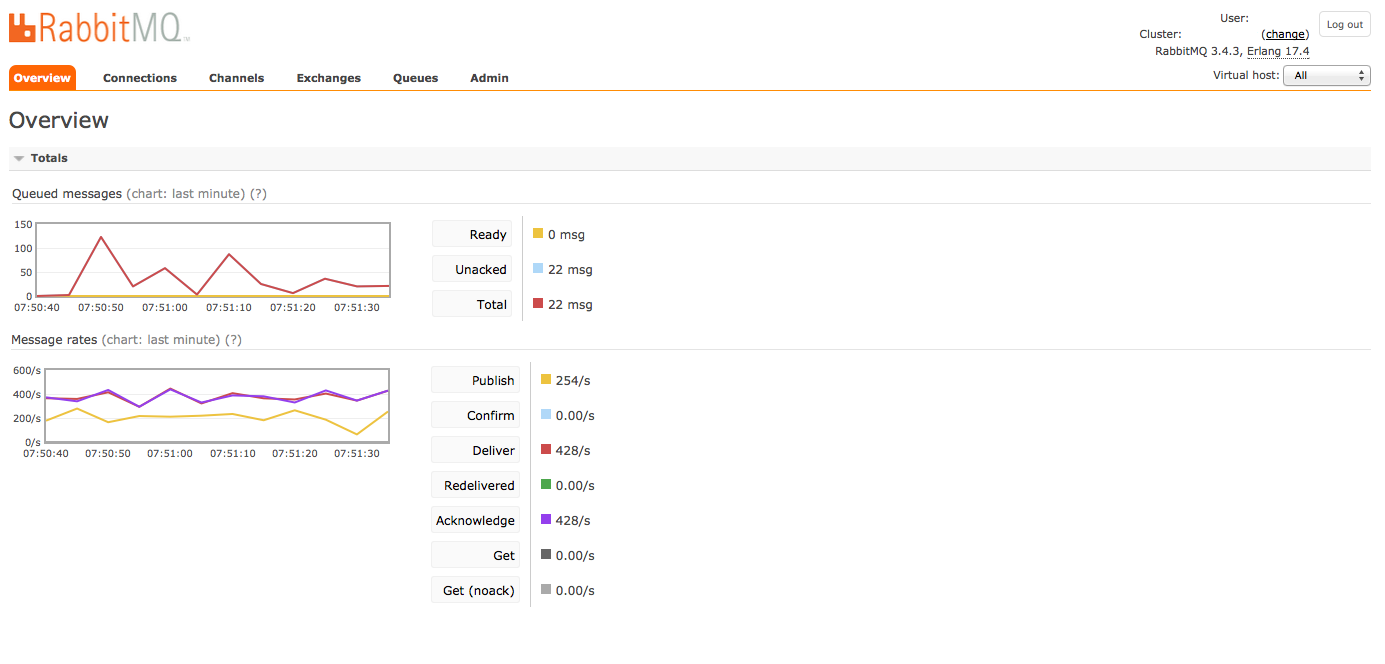
\includegraphics[width=\linewidth]{images/rabbitmq-monitoring.png}}
\caption{RabbitMQ management UI showing messages queued and message data rates\cite{www-rabbitmq-Johan}}
\label{fig:false-color}
\end{figure}

\section{Licensing}
RabbitMQ is licensed under Mozilla Public License(MPL) and GPL v2
\cite{www-rabbitmq-license}. MPL license \cite{www-mpl-license} allows "for free
use, modification, distribution, and "exploit[ation]" of the work, but does not
grant the licensee any rights to a contributor's trademarks".

\section{Use Cases}
RabbitMQ messaging can be useful for applications which require asynchronous
messaging i.e. an application initiates a task by posting a message to RabbitMQ,
it does not have to wait for the task to get completed. Application can
periodically check for the status of completion of the task. RabbitMQ can scale
up as the data needs of the application grow, by just adding additional nodes to
the RabbitMQ cluster. When applications run as micro-services in a containerized
environment, RabbitMQ is useful to communicate and share data between different
services. RabbitMQ can be managed separately using management Web UI, CLI tool
and REST API. This decouples the messaging layer from application and makes the
overall design robust. 

\section{Conclusion}
RabbitMQ is an open source platform and provides a robust messaging platform for
applications. It provides simple manageability decoupling with the application.
RabbitMQ can scale well when application demand increases. It can handle more
data by adding more nodes to the cluster. Based on tests
\cite{jones2011rabbitmq} conducted on RabbitMQ with set of 4K(4096) and 16K
(16384) messages, the performance of RabbitMQ on multi node cluster decreases in
comparison with single node cluster to reach a threshold and then becomes
stable. This decrease in performance can be primarily accounted due to
replication between nodes in the cluster. These tests were conducted on
combination of single publisher and single subscriber, multiple publishers and
single subscriber, multiple publishers and multiple subscribers. Due to time
constraints there is no concrete conclusion to these test and numbers. Further
testing should be conducted on a bigger cluster i.e. more nodes and for longer
duration to produce more consistent results.

\section*{Acknowledgements}
Special thanks to Professor Gregor von Laszewski, Dimitar Nikolov and all
associate instructors for all help and guidance related to latex and bibtex,
scripts for building the project, quick and timely resolution to any technical
issues faced. The paper is written during the course  {I524: Big Data and Open
Source Software Projects, Spring 2017} at Indiana University Bloomington.

\medskip

% Bibliography
% \bibliographystyle{unsrt}
\bibliography{references}

\end{document}
